In this chapter explain the basics of rigid body dynamics simulation.

\section{Problem statement}
Physics simulation is a complex and vast problem. 

\section{Principles of rigid body dynamics simulation}
The section is heavily inspired by \cite{bender2014interactive}.
The basic idea behind the simulation of physics on a computer is to discretize time and apply the laws of newton to each object in the scene and integrate their acceleration during the timestep. When objects collide, collision.

A rigid body is an idealized solid object which will never change its shape, even under high forces.

\begin{figure}[htp]
\center
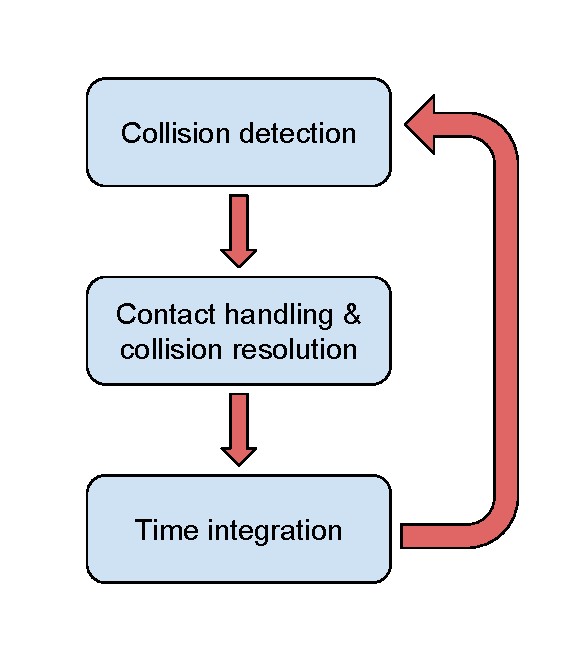
\includegraphics[width=0.3\textwidth]{figures/star_simul_loop}
\caption[Simulation loop]{Simulation loop}
\label{fig:star_simul_loop}
\end{figure}

